%!TEX root = ../report.tex

% 
% Architecture
% 
% (2/3pgs)
\section{Architecture}
\label{sec:architecture}

This section presents \emph{ViewZone}, our proposed solution for TrustZone-enabled devices which supports trusted display for critical Android applications which handle privacy sensitive data. Protected application data may take several formats, either being images or straight plain text files. This flexibility allows app developers to easily create several basic secure applications such as a secure password viewer, a sensitive image display and a sensitive document viewer, without ever being at risk of disclosure by a compromised full-featured OS.

% ARQUITECTURA
\begin{figure}[t!]
	\centering
	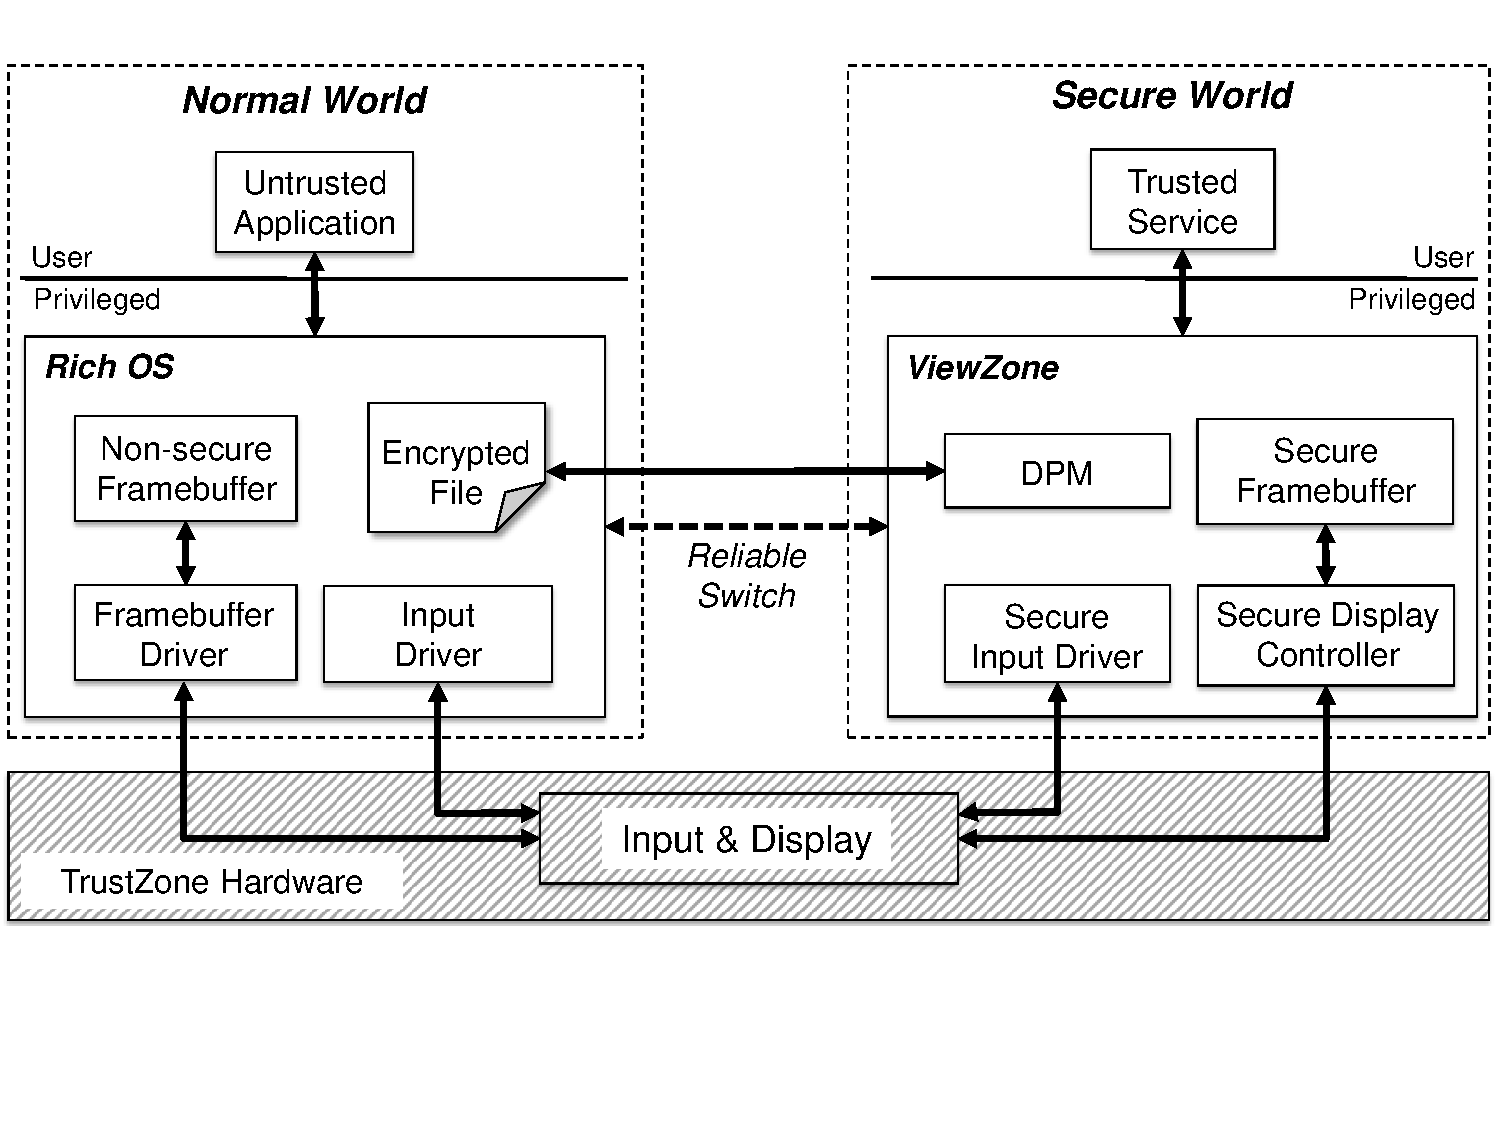
\includegraphics[width=0.9\textwidth]{img/viewzone_architecture.pdf}
	\caption{ViewZone's Architecture}
	\label{fig:viewzone_architecture}
\end{figure}

%\paragraph{\textbf{Architecture}}
Figure~\ref{fig:viewzone_architecture} represents the components and mechanisms which comprise \emph{ViewZone}'s architecture. A typical execution flow of a \emph{ViewZone} applications is as follows: an untrusted application running in the rich OS uses \emph{ViewZone} as a trusted service in the secure domain. This untrusted app loads an encrypted file, whose content is only accessible by the secure world, into a shared memory region. This allows the \ac{DPM} to securely copy the encrypted file to secure memory so it can be decrypted and later displayed to the user. The \ac{DPM} looks into the shared memory region only when the reliable switch is triggered by a secure \ac{NMI} hardware interrupt, thus assuring the subsequent operations are executed by the secure side and the content displayed is authentic.

Once the \ac{DPM} has access to the sensitive file content, the secure display controller copies the non-secure framebuffer to the secure framebuffer and the content of the sensitive file is integrated with that of the original framebuffer, giving the impression of integrated user interface between both domains. This means the trusted service can display content as it would be displayed by the original rich OS interface. When another \ac{NMI} interrupt is triggered, the secure framebuffer is cleared and the control returns to the rich OS.

In order to support secure display as a service for Android applications and maintain a small trusted computing base, \emph{ViewZone} must feature only the strictly necessary components for it to work, and even these components must be designed and built with intelligent and conservative development strategies. Moreover, \emph{ViewZone} must allow for an integrated environment with Android to provide a transparent security environment for critical applications without compromising the system's usability. To support the described features, this project must fulfil the goals of assuring the necessary security policies such as trusted display, confidentiality, integrity and authenticity of data stored in the untrusted world, and be developer friendly in order to be easily deployable. The following paragraphs describe how these goals will be supported in \emph{ViewZone}.

\paragraph{\textbf{Trusted User Interface}}
Trusted services must support secure display so the data from the trusted application cannot be eavesdropped by the rich operating system. To achieve this, a secure display controller must be implemented to securely copy the image from a secure framebuffer to the display device, where the framebuffer stores the image to be displayed. By having different framebuffers for the secure and normal domains, \emph{ViewZone} can prevent potential data leakage, as the secure framebuffer is reserved for use in the secure world. Moreover, because resources such as the video card and display screen are usually shared by both domains, the reliable display controller must be able to correctly program both resources. With this mechanism there is a guarantee that the information displayed to the user is authentic.

\paragraph{\textbf{Secure World-Switching}}

A big limitation of some systems described in section~\ref{sec:relatedWork} is world-switching based on software interrupts, which allow denial-of-service attacks by a malicious rich OS that may sabotage inter-world calls responsible for the world switch. To mitigate such attacks, hardware interrupts responsible for the world-switching mechanism were implemented by the authors of TrustOTP~\cite{sun2015trustotp} and TrustDump~\cite{sun2015reliable} in these systems. \ac{NMI} are hardware interrupts that cannot be ignored by standard interrupt masking techniques. These are typically used to signal attention for non-recoverable hardware errors, but can be used in order to feature secure world-switches between the normal and secure world domains. With these interrupts the user can be guaranteed of an inter-world switch and that the operations dependent of this world-switch are authentic, this is because the secure domain is non-reentrant, meaning that after the system enters the secure domain, the system will switch back to the rich OS only when \emph{ViewZone} explicitly triggers the switch.

\paragraph{\textbf{Secure File Handling}}

%ideia é conseguir ter coisas guardadas no mundo inseguro mas que apenas o viewzone tem acesso
% Sobre a chave, podes adicionar um parágrafo que terá precisamente que referir o problema da chave, e de como esta é aprovisionada. Uma solução inicail que podes referir é que a chave pode já vir de fábrica e que existe uma chave pública associada que pode ser usada para enviar conteúdos cifrados para a ViewZone. Dizer que depois a ViewZone deverá também suportar protocolos criptográficos para renovação da chave.

In order for the sensitive information to be inaccessible by the rich operating system, the file which contains such information must be encrypted. This encryption must be leveraged so that the file is not understandable by the full-featured operating system but is readable by the \emph{ViewZone} service. To achieve this \emph{ViewZone} must  

%In order to bypass the physical limitations of storage in the secure world domain a different strategy must be implemented to support secure storage of large files. Inspired by the work which culminated on the development of DroidVault~\cite{li2014droidvault}, secure storage is possible by enabling large files to be stored in the untrusted domain. To achieve this goal \emph{ViewZone} must implement, similarly to what is done in DroidVault, a \ac{DPM}, which is the secure module for data operations. A file can be created inside \emph{ViewZone}, or downloaded from a remote server, and encrypted with a key generated in the secure side, or known by it. This way, sensitive data is encrypted before leaving \emph{ViewZone} and is never disclosed to the Android OS. Moreover, \ac{DPM} can verify if a client application running in Android (front-end of the \emph{ViewZone} trusted service) is the owner of the encrypted data. If it is then the \ac{DPM} is responsible for loading the corresponding file in the secure world domain so it can be securely managed by the trusted application. The \ac{DPM} assures the confidentiality and integrity of sensitive data in \emph{ViewZone} and allows for large files to be securely stored in the untrusted domain of a TrustZone-enabled mobile device.

\paragraph{\textbf{Developer Friendly}}

\emph{ViewZone} should allow for an easy deployment of critical applications using the trusted display service. The developer should not have to handle low level primitives regarding device drives, framebuffers or display controllers, as this is to be done by \emph{ViewZone}. As such, developers should leverage an API which, by communicating with \emph{ViewZone}'s service running in the secure domain, is capable of registering for the secure service, send the encrypted file to be displayed by the secure service and store it securely, with the necessary credentials, in the Android filesystem.

% DIGO QUE ISTO EXISTE MAS NAO EXPLICO COMO FUNCIONA